\documentclass[oneside,a4paper,11pt,explicit]{book}
\usepackage[utf8]{inputenc}
\usepackage{icecream}
\usepackage[english]{babel}
\addto\captionsenglish{\renewcommand{\chaptername}{}}
\usepackage[accsupp]{axessibility}  % improves PDF readability for those with disabilities.
\usepackage[colorlinks = true,urlcolor  = blue,linkcolor = blue]{hyperref}
\usepackage{setspace}
\usepackage{listings}
\usepackage[most]{tcolorbox}
\usepackage{minitoc}
\usepackage{multicol}


\renewcommand{\mtifont}{\large\sffamily}
\renewcommand{\mtcfont}{\small\sffamily}
\renewcommand{\mtcSfont}{\small\sffamily}
\renewcommand{\mtcSSfont}{\small\sffamily}
\renewcommand{\mtcSSSfont}{\small\sffamily}
\mtcsetpagenumbers{minitoc}{off} % turn off page numbering in minitocs
\addto{\captionsenglish}{% Making babel aware of special titles
	\renewcommand{\mtctitle}{Quick Links To Sections}
}
\setlength{\fboxrule}{5pt}
\setlength{\fboxsep}{4pt}

\definecolor{IceCreamLeaf}{HTML}{58743b}
\definecolor{IceCreamOrbit}{HTML}{732e00}
\definecolor{MACred}{rgb}{0.803921568627451, 0.3607843137254902, 0.3607843137254902}

\title{I.C.E.C.R.E.A.M. Tutorials}
\subtitle{\small Observing Earth from Above (Env 329) v24.06  \\
	\small Schmid College of Science and Technology, Chapman University}
\date{\today}

%% DOCUMENT
\setstretch{1.25}
\makeatletter
\begin{document}

\setcounter{tocdepth}{3}
\setcounter{minitocdepth}{3}
\dominitoc
\faketableofcontents

\setcounter{chapter}{3} %Insert (Tutorial Number-1) Here; example for tutorial 4, enter 3

\chapter{Accessing Remote Sensing Data With A$\rho\rho$EEARS} %Enter Tutorial Name Here

\vspace{-2em}

\minitoc

\hrule

\vspace{1em}

\begin{tcolorbox}[enhanced,frame style image=blueshade.png,
	opacityback=0.75,opacitybacktitle=0.25,
	colback=blue!5!white,colframe=blue!75!black,title={\Large \textbf{Objectives:}}]
	\large
	\begin{enumerate}
		\item Access the A$\rho\rho$EEARS website and practice using its interface.
		\item Download ECOSTRESS land surface temperature data from A$\rho\rho$EEARS.
	\end{enumerate}
\end{tcolorbox}

\clearpage

%%%%%%%%%%%%%%%%%%%%%%%%%%%%%%%%%% Change Header to Have a Smaller Logo for Remainder of the Document
\fancyhead{}
\fancyhead[C]{\begin{tikzpicture}[overlay, remember picture]
		\fill[Blue2] (current page.north west) rectangle ($(current page.north east)+(0,-1in)$);
		\node[anchor=north west, text=white, font=\Large, minimum size=1in, inner xsep=5mm, align=left] at (current page.north west) {\bf{\MakeUppercase{\@title}}\\\@subtitle};
		\node[anchor=north east, minimum size=1in, inner xsep=5mm] at (current page.north east) {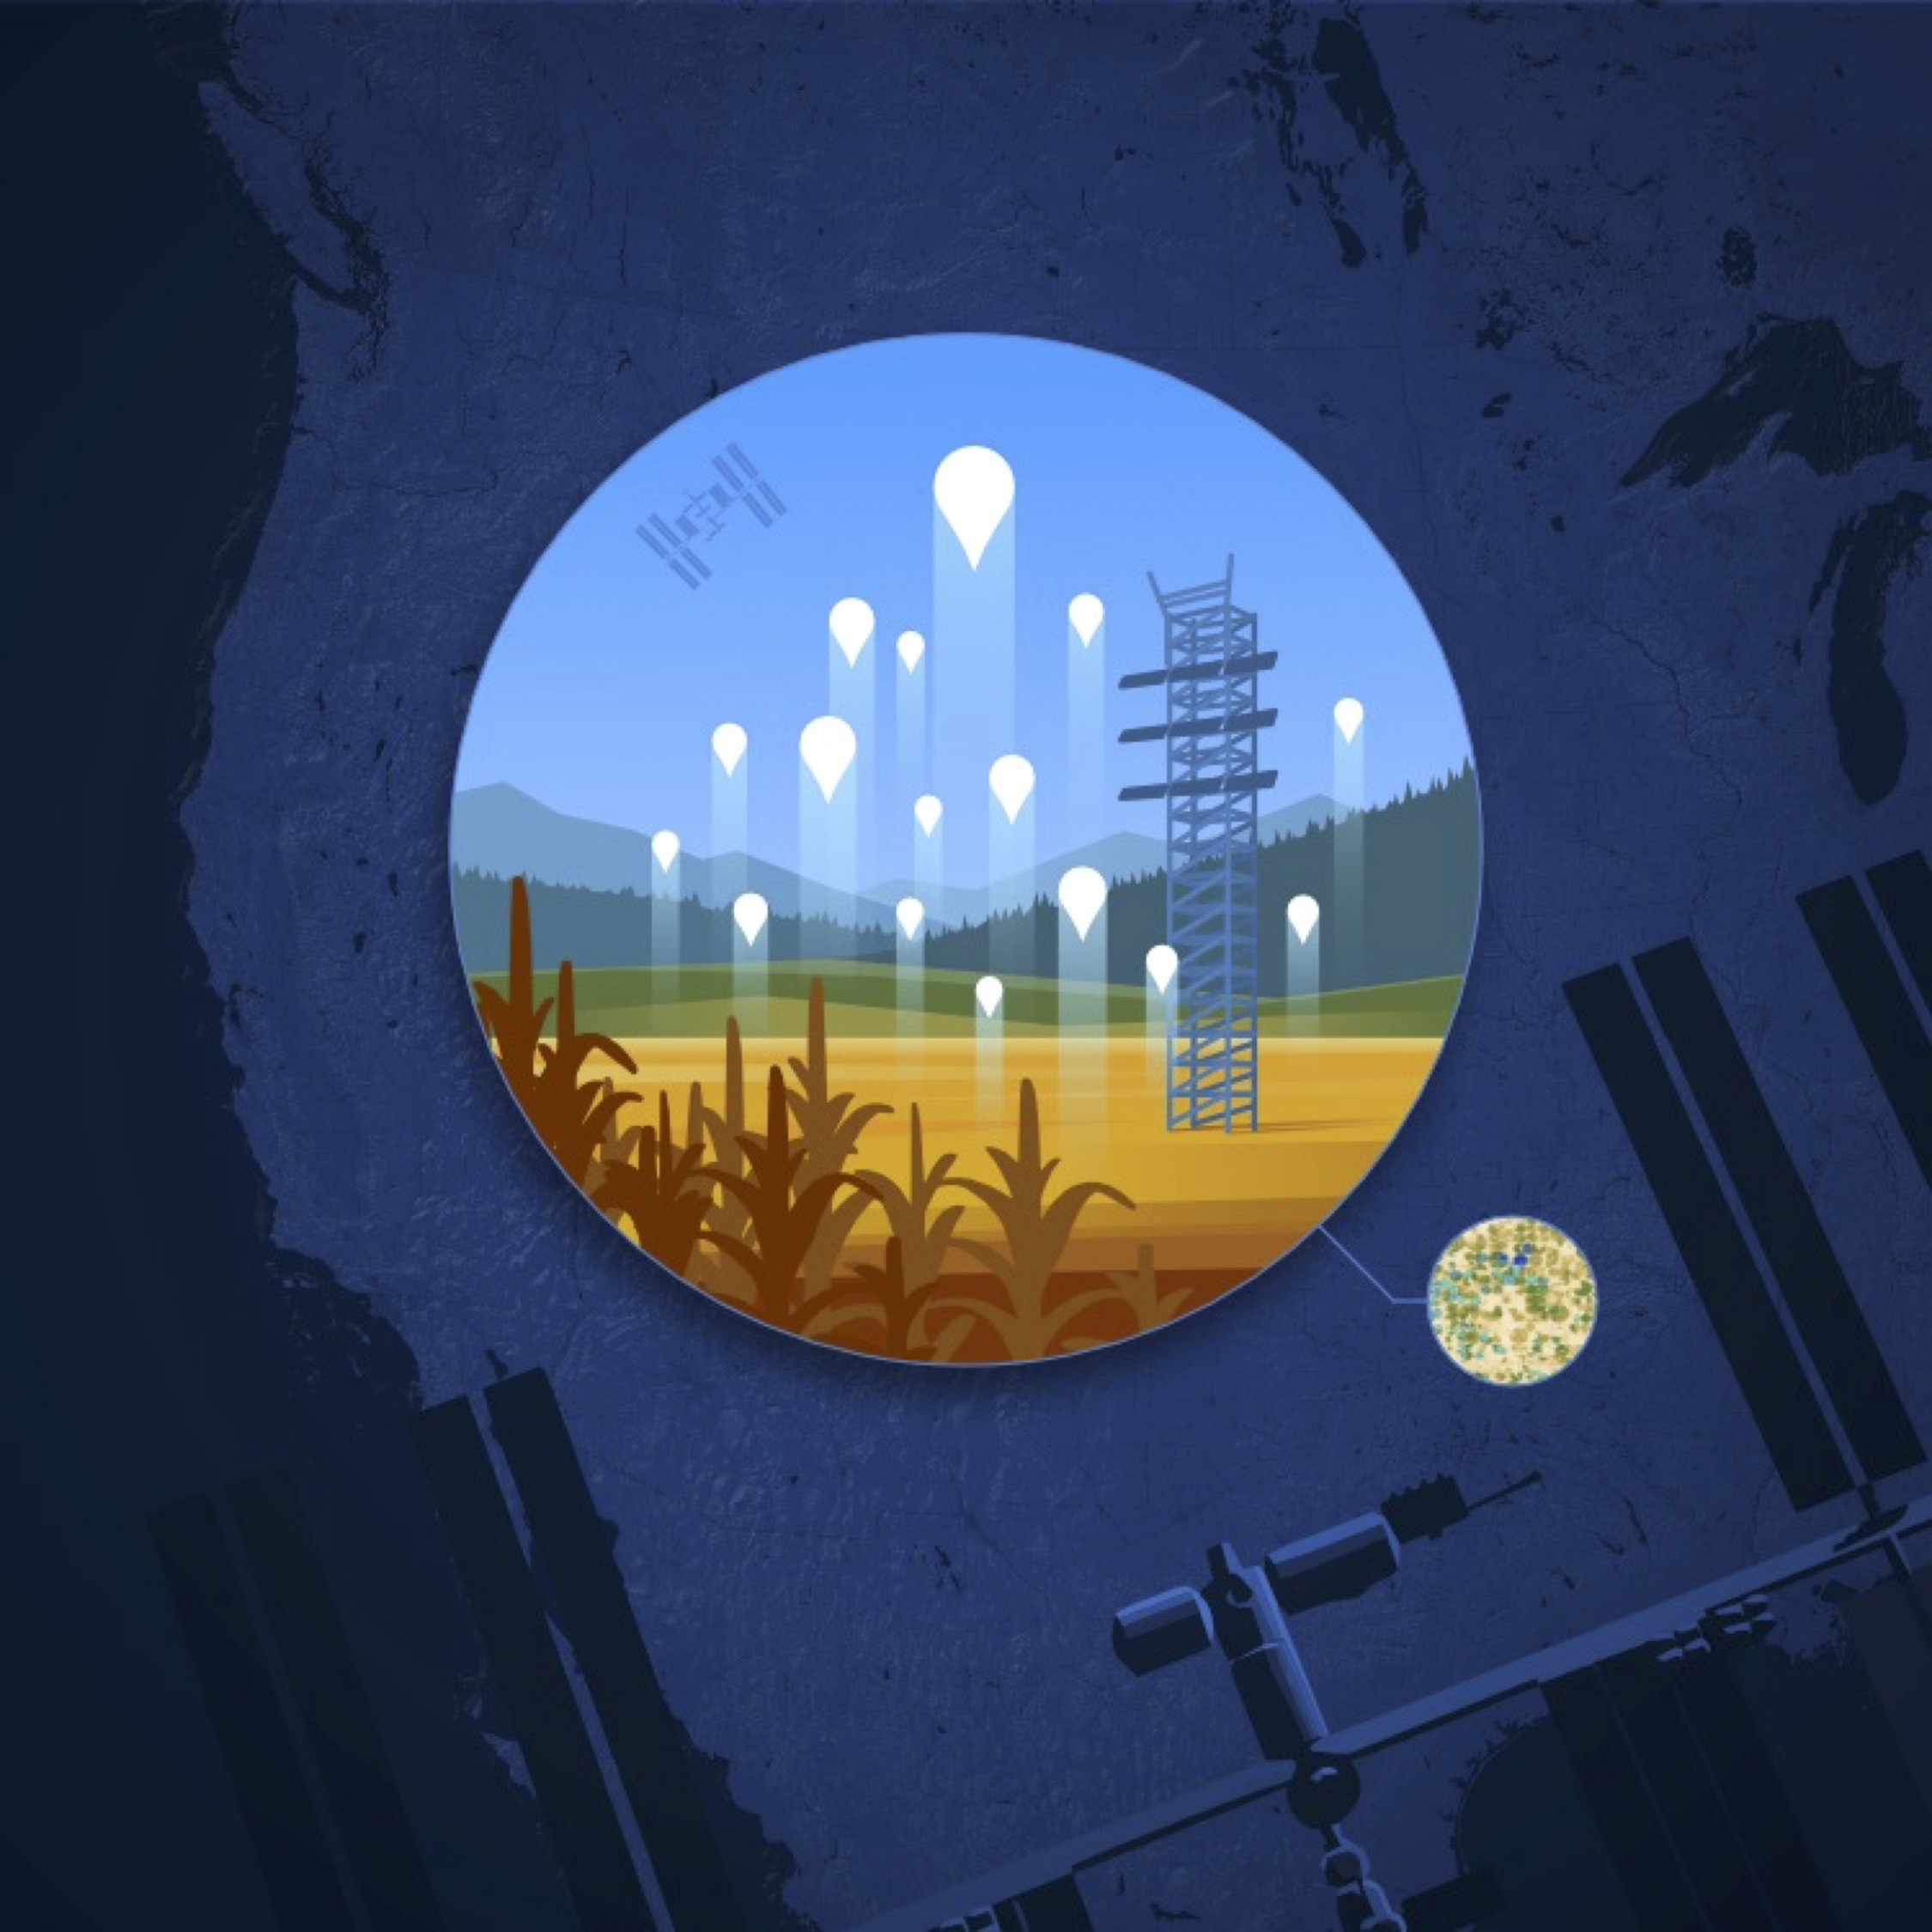
\includegraphics[scale=.03]{ECOSTRESS-BASE.jpg}};\end{tikzpicture}}
%%%%%%%%%%%%%%%%%%%%%%%%%%%%%%%%%%

\noindent\fbox{\begin{minipage}{.9665\textwidth}
			
	\vspace{1em}
	\begin{center}
		\textbf{\Large \underline{Motivation For Today's Tutorial: Heat in Death Valley}}
	\end{center}
	
	\addcontentsline{toc}{section}{Motivation : Death Valley}

	\vspace*{-1 em}
	
	\centerline{\includegraphics[width=\textwidth]{DeathValleySignECOSTRESS.png}}

	ECOSTRESS primarily measures land surface temperatures (LST), so let's look at the thermometer at one of the hottest places on the planet: Death Valley, California. The highest recorded ground temperature was verified at 201 °F on July 15, 1972. However, it recently had one of the hottest months on record, where air temperatures reached upwards of 128 °F in July of 2023. We are going to download the land surface temperature data from ECOSTRESS for those days to see how close it was to breaking the surface temperature record.
	
	\kulbox{\textbf{NOTE:} ECOSTRESS launched on July 9, 2018, so as you think about potential projects, you cannot design a project that requires data before that date.}

\end{minipage}}

\section{Welcome Back!} 

Today, we are introducing A$\rho\rho$EEARS, which is short for "The Application for Extracting and Exploring Analysis Ready Samples." A$\rho\rho$EEARS is a web-based application designed to efficiently connect users with geospatial data that has been generated by satellite remote sensing instruments associated with agencies such as NASA and the U.S. Geological Survey. Satellite data is often available through different platforms, but today we are going to use A$\rho\rho$EEARS to access data from the \href{https://ecostress.jpl.nasa.gov/}{ECOsystem Spaceborne Thermal Radiometer Experiment on Space Station (ECOSTRESS)} instrument. 

1. To begin, visit \url{https://appeears.earthdatacloud.nasa.gov/}. Click the \textit{Sign In} button to register for an Earthdata account, or login if you already have an account.

\vspace{.5em}

\centerline{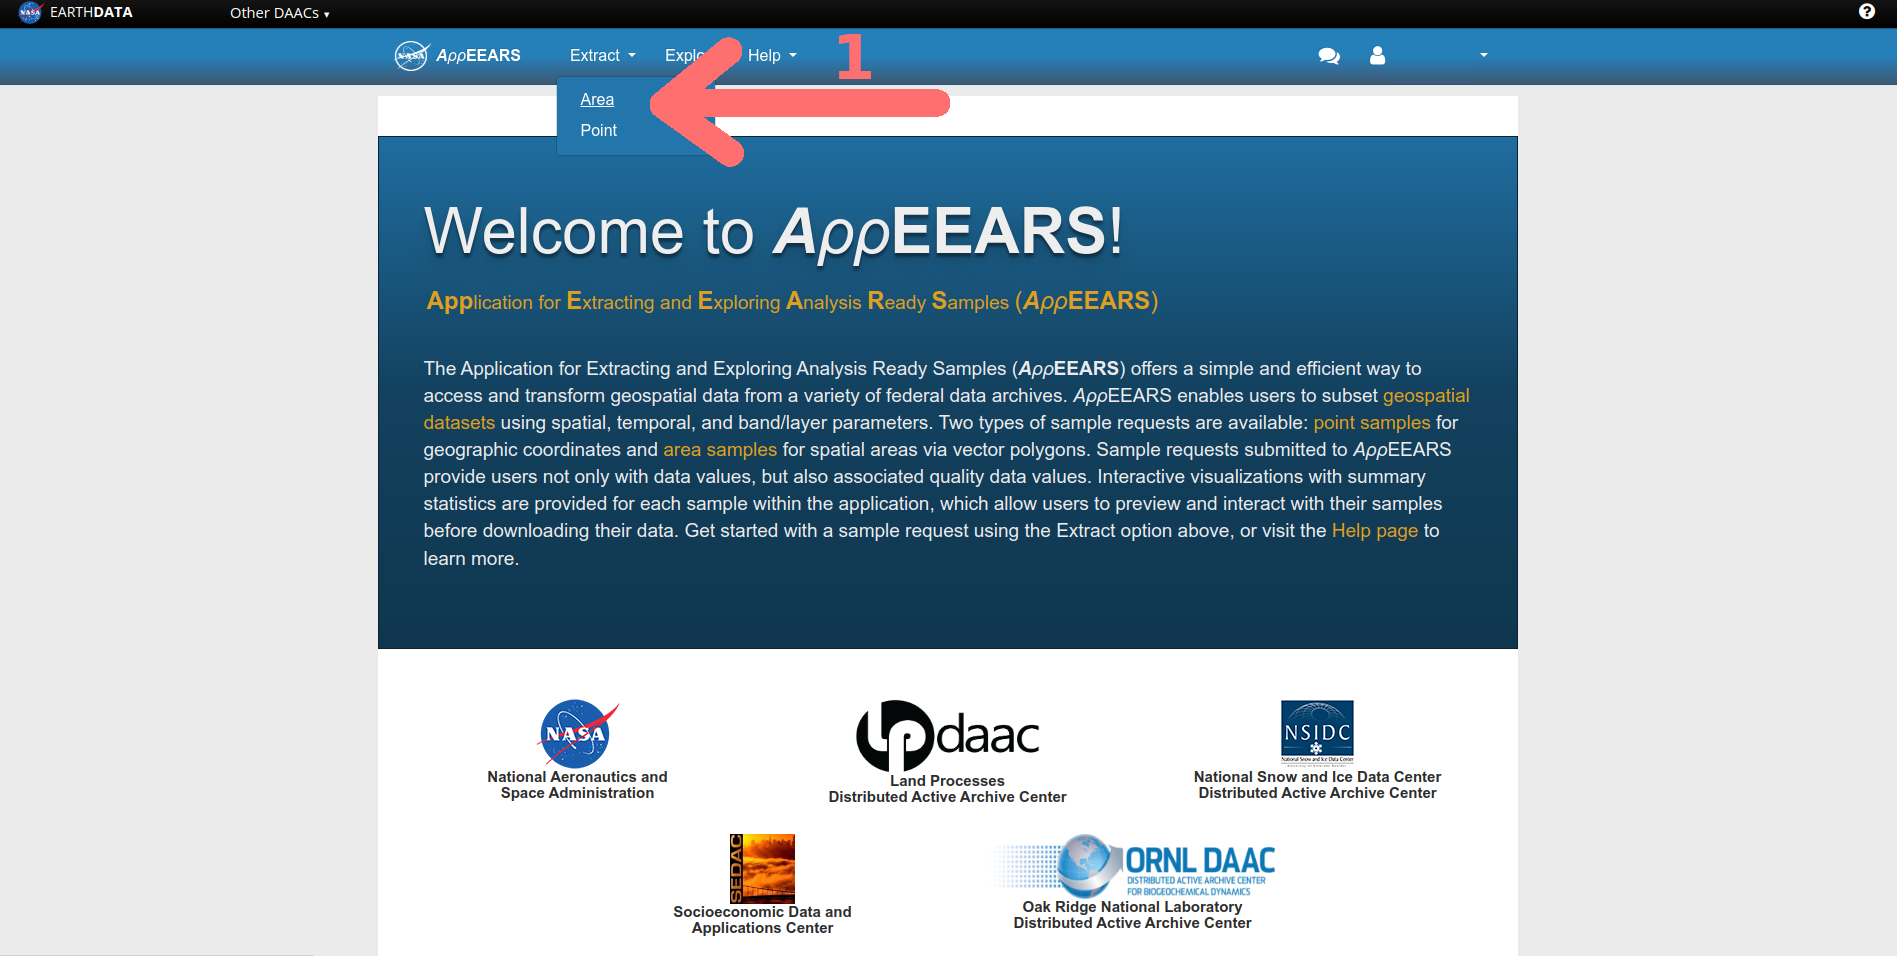
\includegraphics[width=\textwidth]{AppEEARShome.png}}

A$\rho\rho$EEARS allows you to download either point (i.e., data from a single pixel at a given latitude/longitude) or area (i.e. all pixels that fall within a given area defined by a polygon). It also allows you to choose the time interval for the data and the type of data you wish to request.  

\section{Create A Request}
2. To access satellite data, use the \textit{Extract} dropdown menu to select \textit{Area}. 

3. Select \textit{Start a new request} to request data for a new area and a new period of time.

4. Enter a useful name for the request you are going to submit, such as ``Death Valley Temperature Observations.'' Getting into the habit of assigning unique and relevant names will be useful when you start making many requests for data from A$\rho\rho$EEARS.

\vspace{1em}

Now, we need to specify to A$\rho\rho$EEARS your geographic area of interest (AOI), which in this case is Death Valley National Park. This can be accomplished in a few different ways:

\begin{itemize}
	\item Using the map interface to draw a rectangle or polygon that encompasses your AOI.
	\item Uploading a \href{https://en.wikipedia.org/wiki/Shapefile}{shapefile} that describes your AOI.	
\end{itemize}

Today, we are going to use a shapefile with a polygon (that is, an outline) of the park boundaries that we already drew for you in QGIS.

\vspace{1em}

5. Download the \href{https://jeremydforsythe.github.io/icecream-tutorials/Tutorial4_AccessingRemoteSensingDataWithAppears/DeathValleyNationalPark.zip}{DeathValleyNationalPark.zip} shapefile and save it somewhere you can remember. A folder containing all of the files for this tutorial sounds effective and orderly. 

\centerline{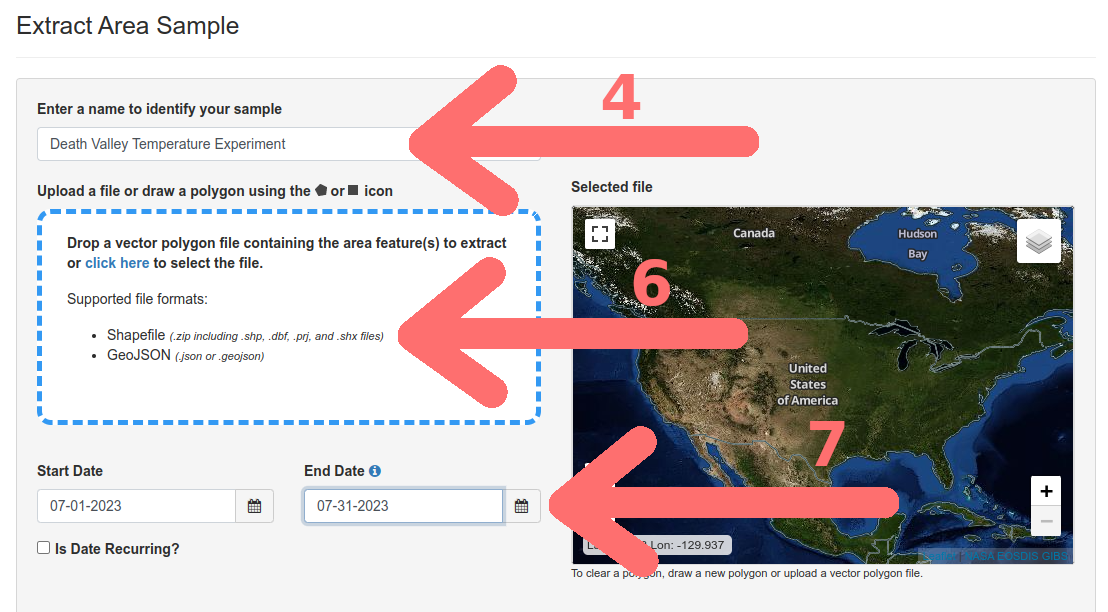
\includegraphics[width=\textwidth]{ExtractDeathValley.png}}

6. Drag and drop (or use the \textit{click here to select the file} link) to upload the shapefile \textbf{DeathValleyNationalPark.zip}. The map should update with a polygon that encompasses Death Valley National Park.

7. Update the \textit{Start} and \textit{End} Date Fields for our month of interest: 07/01/2023 to 07/31/2023

\kulbox{\textbf{NOTE:} While A$\rho\rho$EEARS provides access to a wealth of \href{https://appeears.earthdatacloud.nasa.gov/products}{different data products}, here we are primarily focusing on data from the ECOSTRESS instrument.}

8. Under \textit{Select the layers to include in the sample} type the word ``ECOSTRESS'' and scroll until you can click on \textit{ECOSTRESS Land Surface Temperature \& Emissivity (LST\&E)}. From there, scroll until you see the Land Surface Temperature (\textit{SDS\textunderscore LST}) option. Click on the ``$+$'' sign to add the layer into your cart. Next, clear the current category selection using the small ``x'' to the right of the \textit{ECOSTRESS Land Surface Temperature \& Emissivity (LST\&E)} blue box. Then search for ``Cloud'' and add \textit{Cloud\textunderscore final} from the \textit{ECOSTRESS Cloud Mask Instantaneous} category to your selected layers cart.

\kulbox{\textbf{NOTE:} If you want to learn more about the types and formats of the ECOSTRESS Mission data, you can find all sorts of interesting facts here: \url{https://lpdaac.usgs.gov/data/get-started-data/collection-overview/missions/ecostress-overview/}}

9. Under \textit{Output Options}, we want to use GeoTIFF (Geographic Tagged Image File Format; an image file in which the corresponding geographic information is embedded in the file) and \textit{Native Projection} for projection.

10. Click \textit{Submit} to complete the data request. At the top, you should see a green banner:

\centerline{
\includegraphics[width=\textwidth]{RequestSuccess.png}}

\centerline{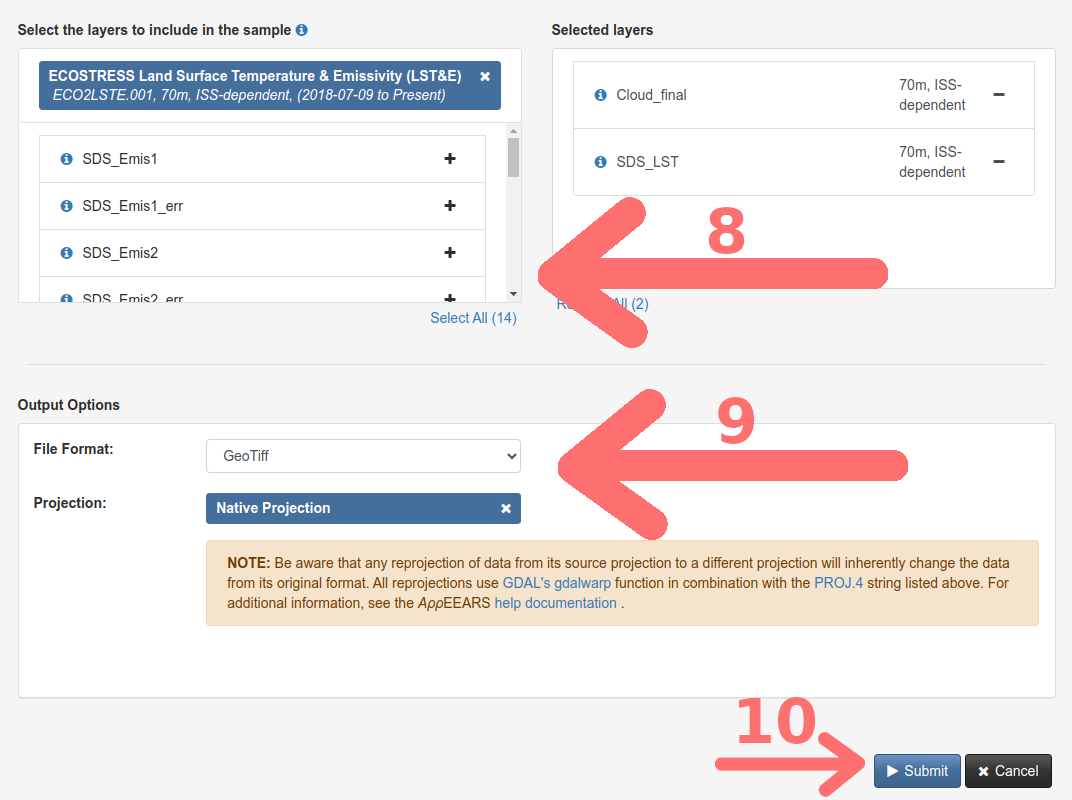
\includegraphics[width=\textwidth]{LayerSettings.png}}

11. You can also track the progress of your request and access the data at \url{https://appeears.earthdatacloud.nasa.gov/explore}. Most small requests will take 15 minutes or less; larger requests can take up to an hour or more. Follow the \textit{Explore} link in your completed request email (or via the Explore menu tab on the A$\rho\rho$EEARS homepage) to access your data.

\kulbox{\textbf{NOTE:} While using the A$\rho\rho$EEARS interface, you will occasionally encounter an error, or the system may be out-of-service for maintenance or updating. If it is the latter, there will be a banner at the top of the A$\rho\rho$EEARS webpage with information about the timeline to restore service. If you encounter an error without a banner present, you can submit a support ticket request help at : \url{https://lpdaac.usgs.gov/lpdaac-contact-us/}.}

\kulbox{\textbf{NOTE:} For these tutorials, we have provided links at the end of each page to the necessary files in the event that the A$\rho\rho$EEARS interface is not functioning.}

\centerline{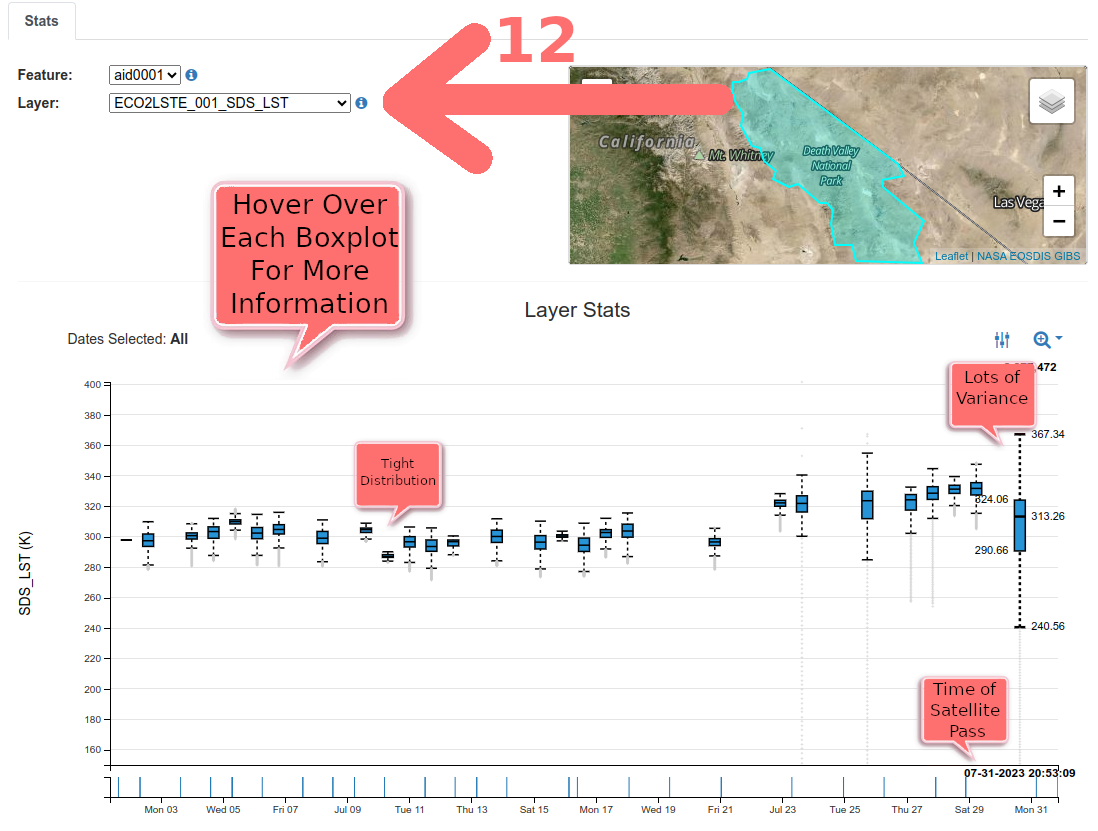
\includegraphics[width=\textwidth]{ExploreLST.png}}

\section{Always Check Your Data} 

12. Before we download the files, we should preview the data using the built-in A$\rho\rho$EEARS visualizations. First, make sure that the Land Surface Temperature (LST) layer is selected. Under \textit{Layer Stats}, you will see a box plot time series of the temperature data on the x-axis of the range of dates and the temperature observed by the instrument for each date (y-axis). For a reminder about what information is encompassed in a boxplot, see the image below. Next, hover over the boxplots in the time series to see all sorts of useful information, including the date and time of day that ECOSTRESS passed overhead collected the data. Although 7/26/2023 had the hottest air temperature of the month, our observations of surface temperature are among the lowest! Why? Have we discovered some new physical property of the desert? Well, no, the ECOSTRESS overpass was simply at 9:49 AM, which was not exactly the hottest part of the day.

\kulbox{\textbf{NOTE:}  ECOSTRESS makes temperature observations on the Kelvin scale and must be converted to Fahrenheit or Celsius.}

\centerline{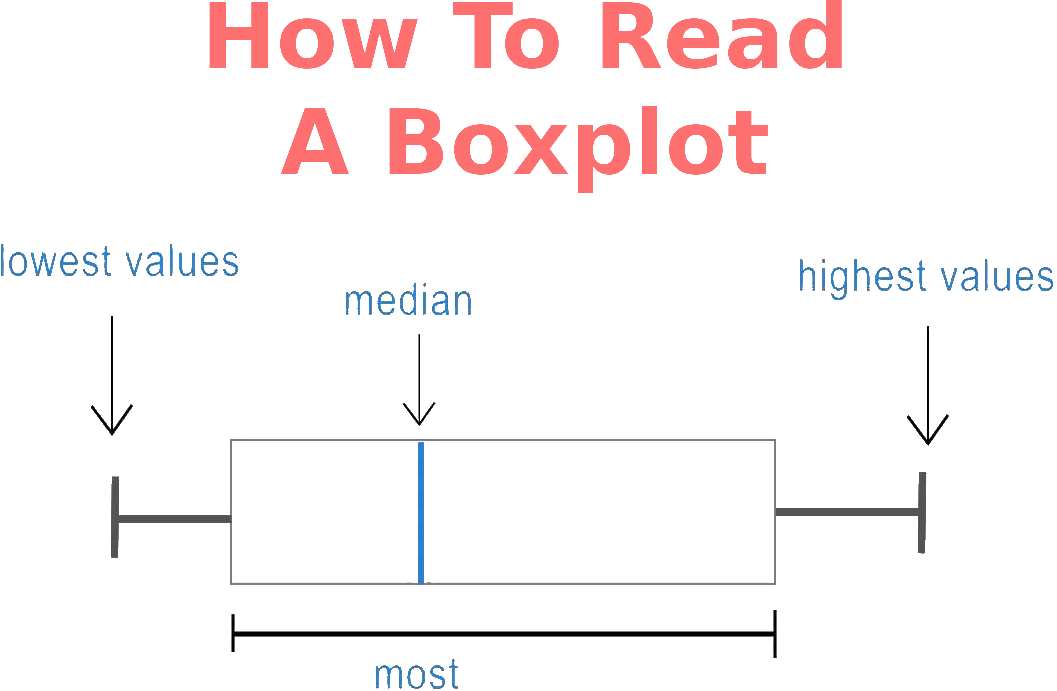
\includegraphics[width=.5\textwidth]{HowToBoxplot.png}}

\begin{tcolorbox}[colback=yellow!5!white,colframe=IceCreamLeaf,title=\textbf{Cloudy Conditions}]
You are likely to notice that the distribution of temperatures for a given \href{https://en.wikipedia.org/wiki/Orbital_pass}{orbital pass} from the instrument is quite variable. In some instances, like on Tuesday, 7/11/2023, all the temperatures are close to the median. On other days, like Monday, 7/31/2023, the temperatures vary considerably. If this was a different locale, it could mean that there is a lot of variation in surface temperatures across this geographic area of interest. However, we know that Death Valley is consistently a hot desert. In this case, it is more likely that there is another culprit: clouds.

\vspace{1em}

\centerline{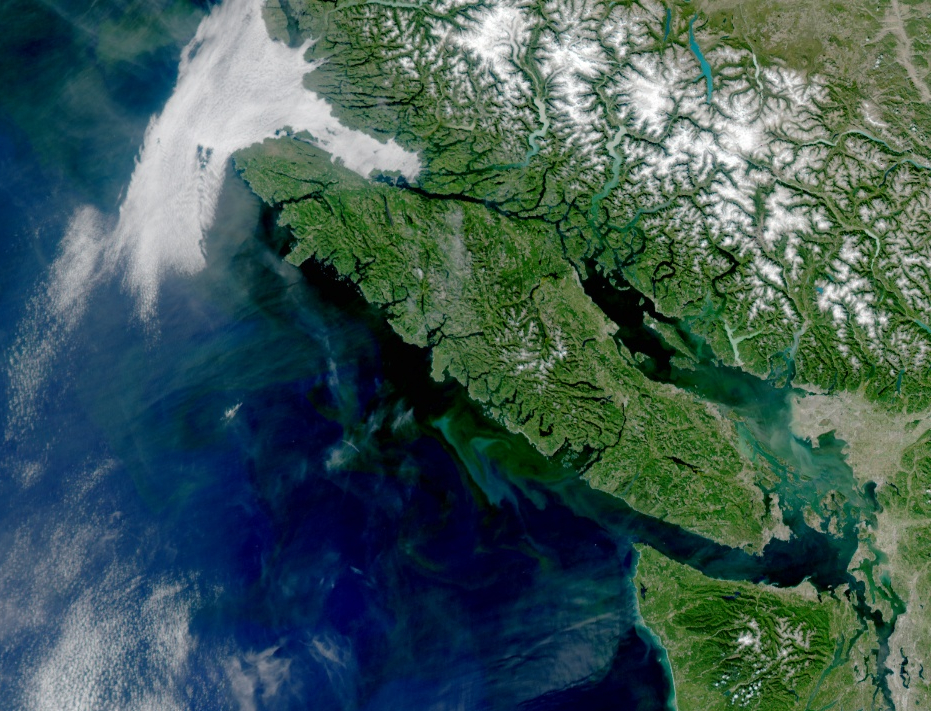
\includegraphics[width=.475\textwidth]{I201625621_250_acor_map_comp.jpg} 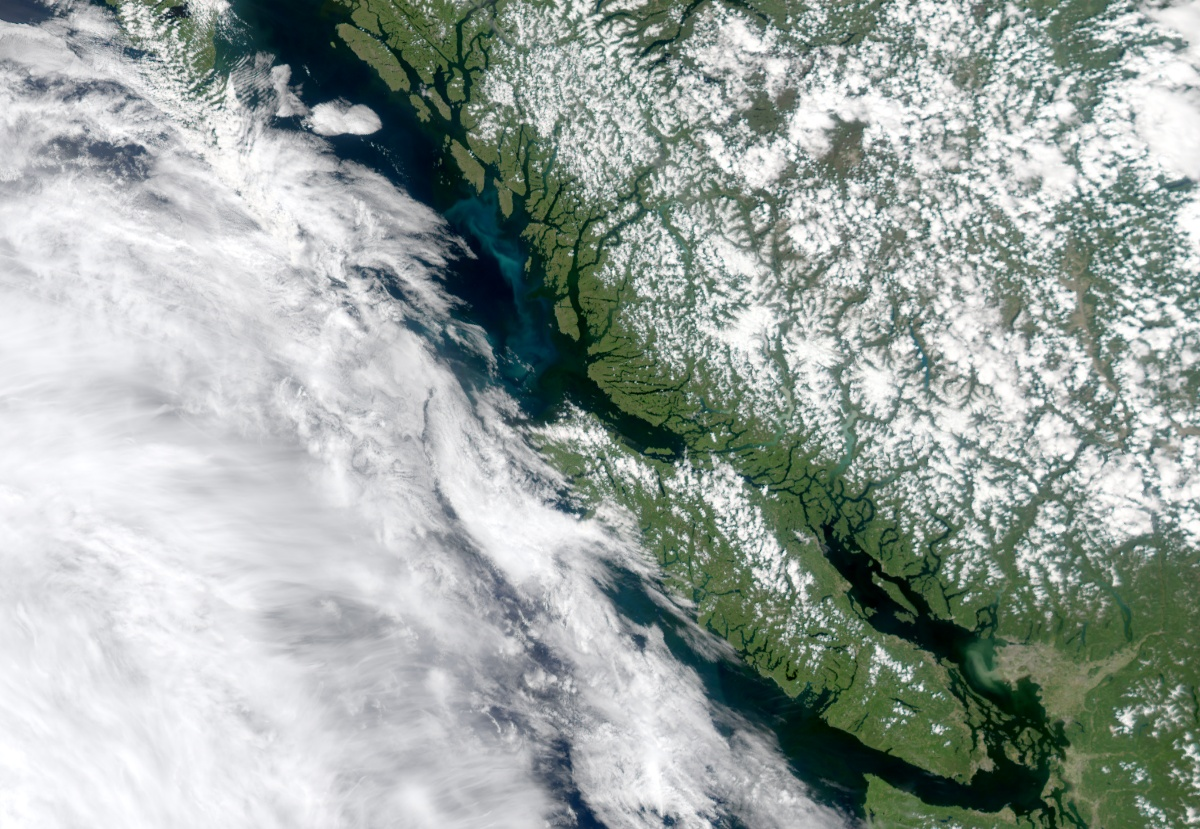
\includegraphics[width=.525\textwidth]{I201517422_250_acor_map_comp.jpg}}

\vspace{1em}

Satellite observations have many advantages, but they cannot accurately make measurements through clouds (see the example above, where NASA's MODIS Satellite captures images of clouds moving over Vancouver Island). To account for this possibility, the ECOSTRESS mission (and others) have built cloud detection algorithms and included those data in A$\rho\rho$EEARS. Checking for the effects of cloud cover on the accuracy and precision of the results is an important part of data quality control and assurance. 
\end{tcolorbox}

13. Change the layer in the built-in A$\rho\rho$EEARS visualizations to Cloud\textunderscore final. Now, we have a different visualization, the output of the cloud detecting algorithm. The bar chart breaks down the percentage of pixels that are clear (blue) and pixels that have clouds (orange). Satellite passes that are free of clouds, or have few clouds, have higher quality data with fewer outliers because there is little interference. To make our map of surface temperatures in Death Valley, let's use data from the hottest cloud free day: 7/28/2023. 

\centerline{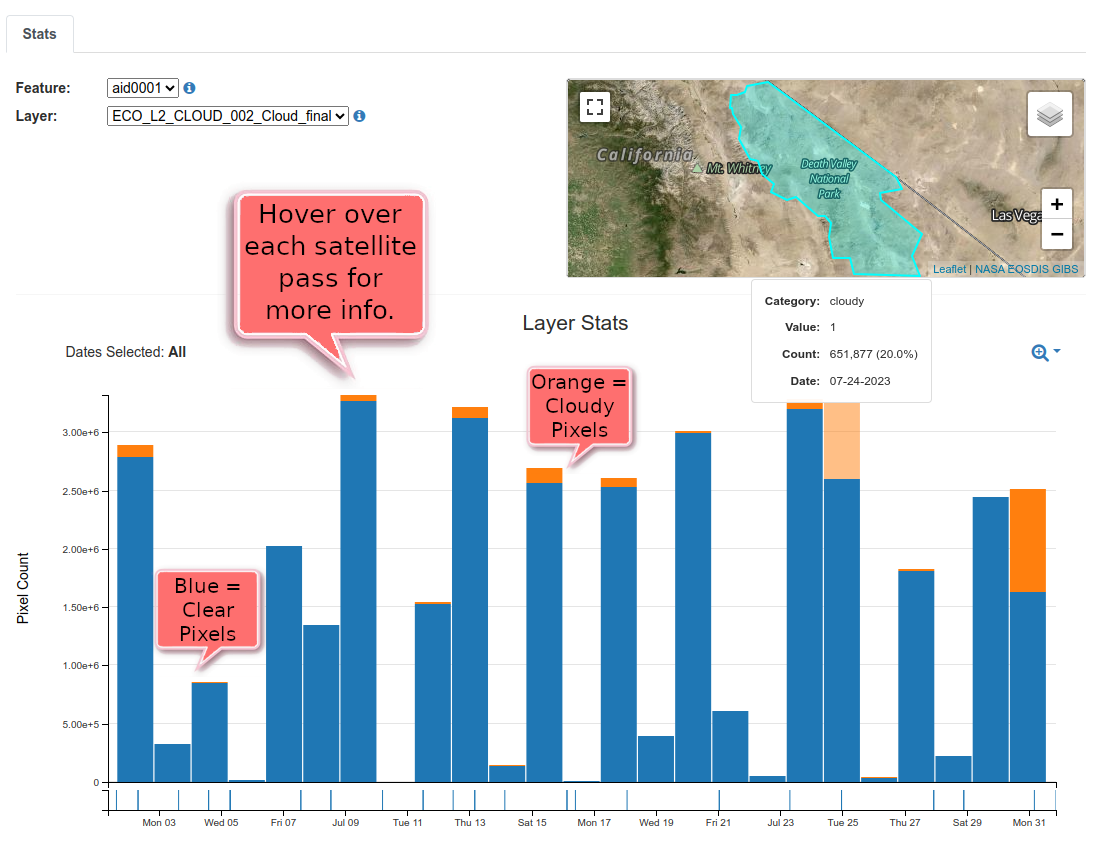
\includegraphics[width=\textwidth]{ExploreClouds.png}}

\section{Downloading Data}

The output data files returned by A$\rho\rho$EEARS have the following naming convention:  

\vspace{.5em}

\small{$<$ProductShortName$>$.$<$Version$>$\textunderscore $<$LayerName$>$\textunderscore doy$<$Year$>$$<$JulianDate$>$\textunderscore $<$AppEEARSFeatureID$>$.$<$FileFormat$>$}

\vspace{.5em}

Example output file name (.tif): 
\begin{itemize}
	\item ECO2LSTE.001\textunderscore SDS\textunderscore LST\textunderscore doy2023209214149\textunderscore aid0001.tif 
\end{itemize}

where: 

    $<$ProductShortName$>$ ................ ECO2LSTE \\
    $<$Version$>$ ................ 001  \\
    $<$LayerName$>$ ................ SDS\textunderscore LST \\
    $<$Year$>$ ................ 2023  \\
    $<$JulianDate$>$ ................ 209  \\
    $<$AppEEARSFeatureID$>$ ................ aid0001 \\
    $<$FileFormat$>$ ................ tif

\vspace{.5em}

In this case, we are primarily concerned with the layer name, which corresponds to our variable of interest (i.e., land surface temperature = \textit{SDS\textunderscore LST}), and with the time of the satellite pass (i.e., Year = 2023, Julian Date = 209).

\centerline{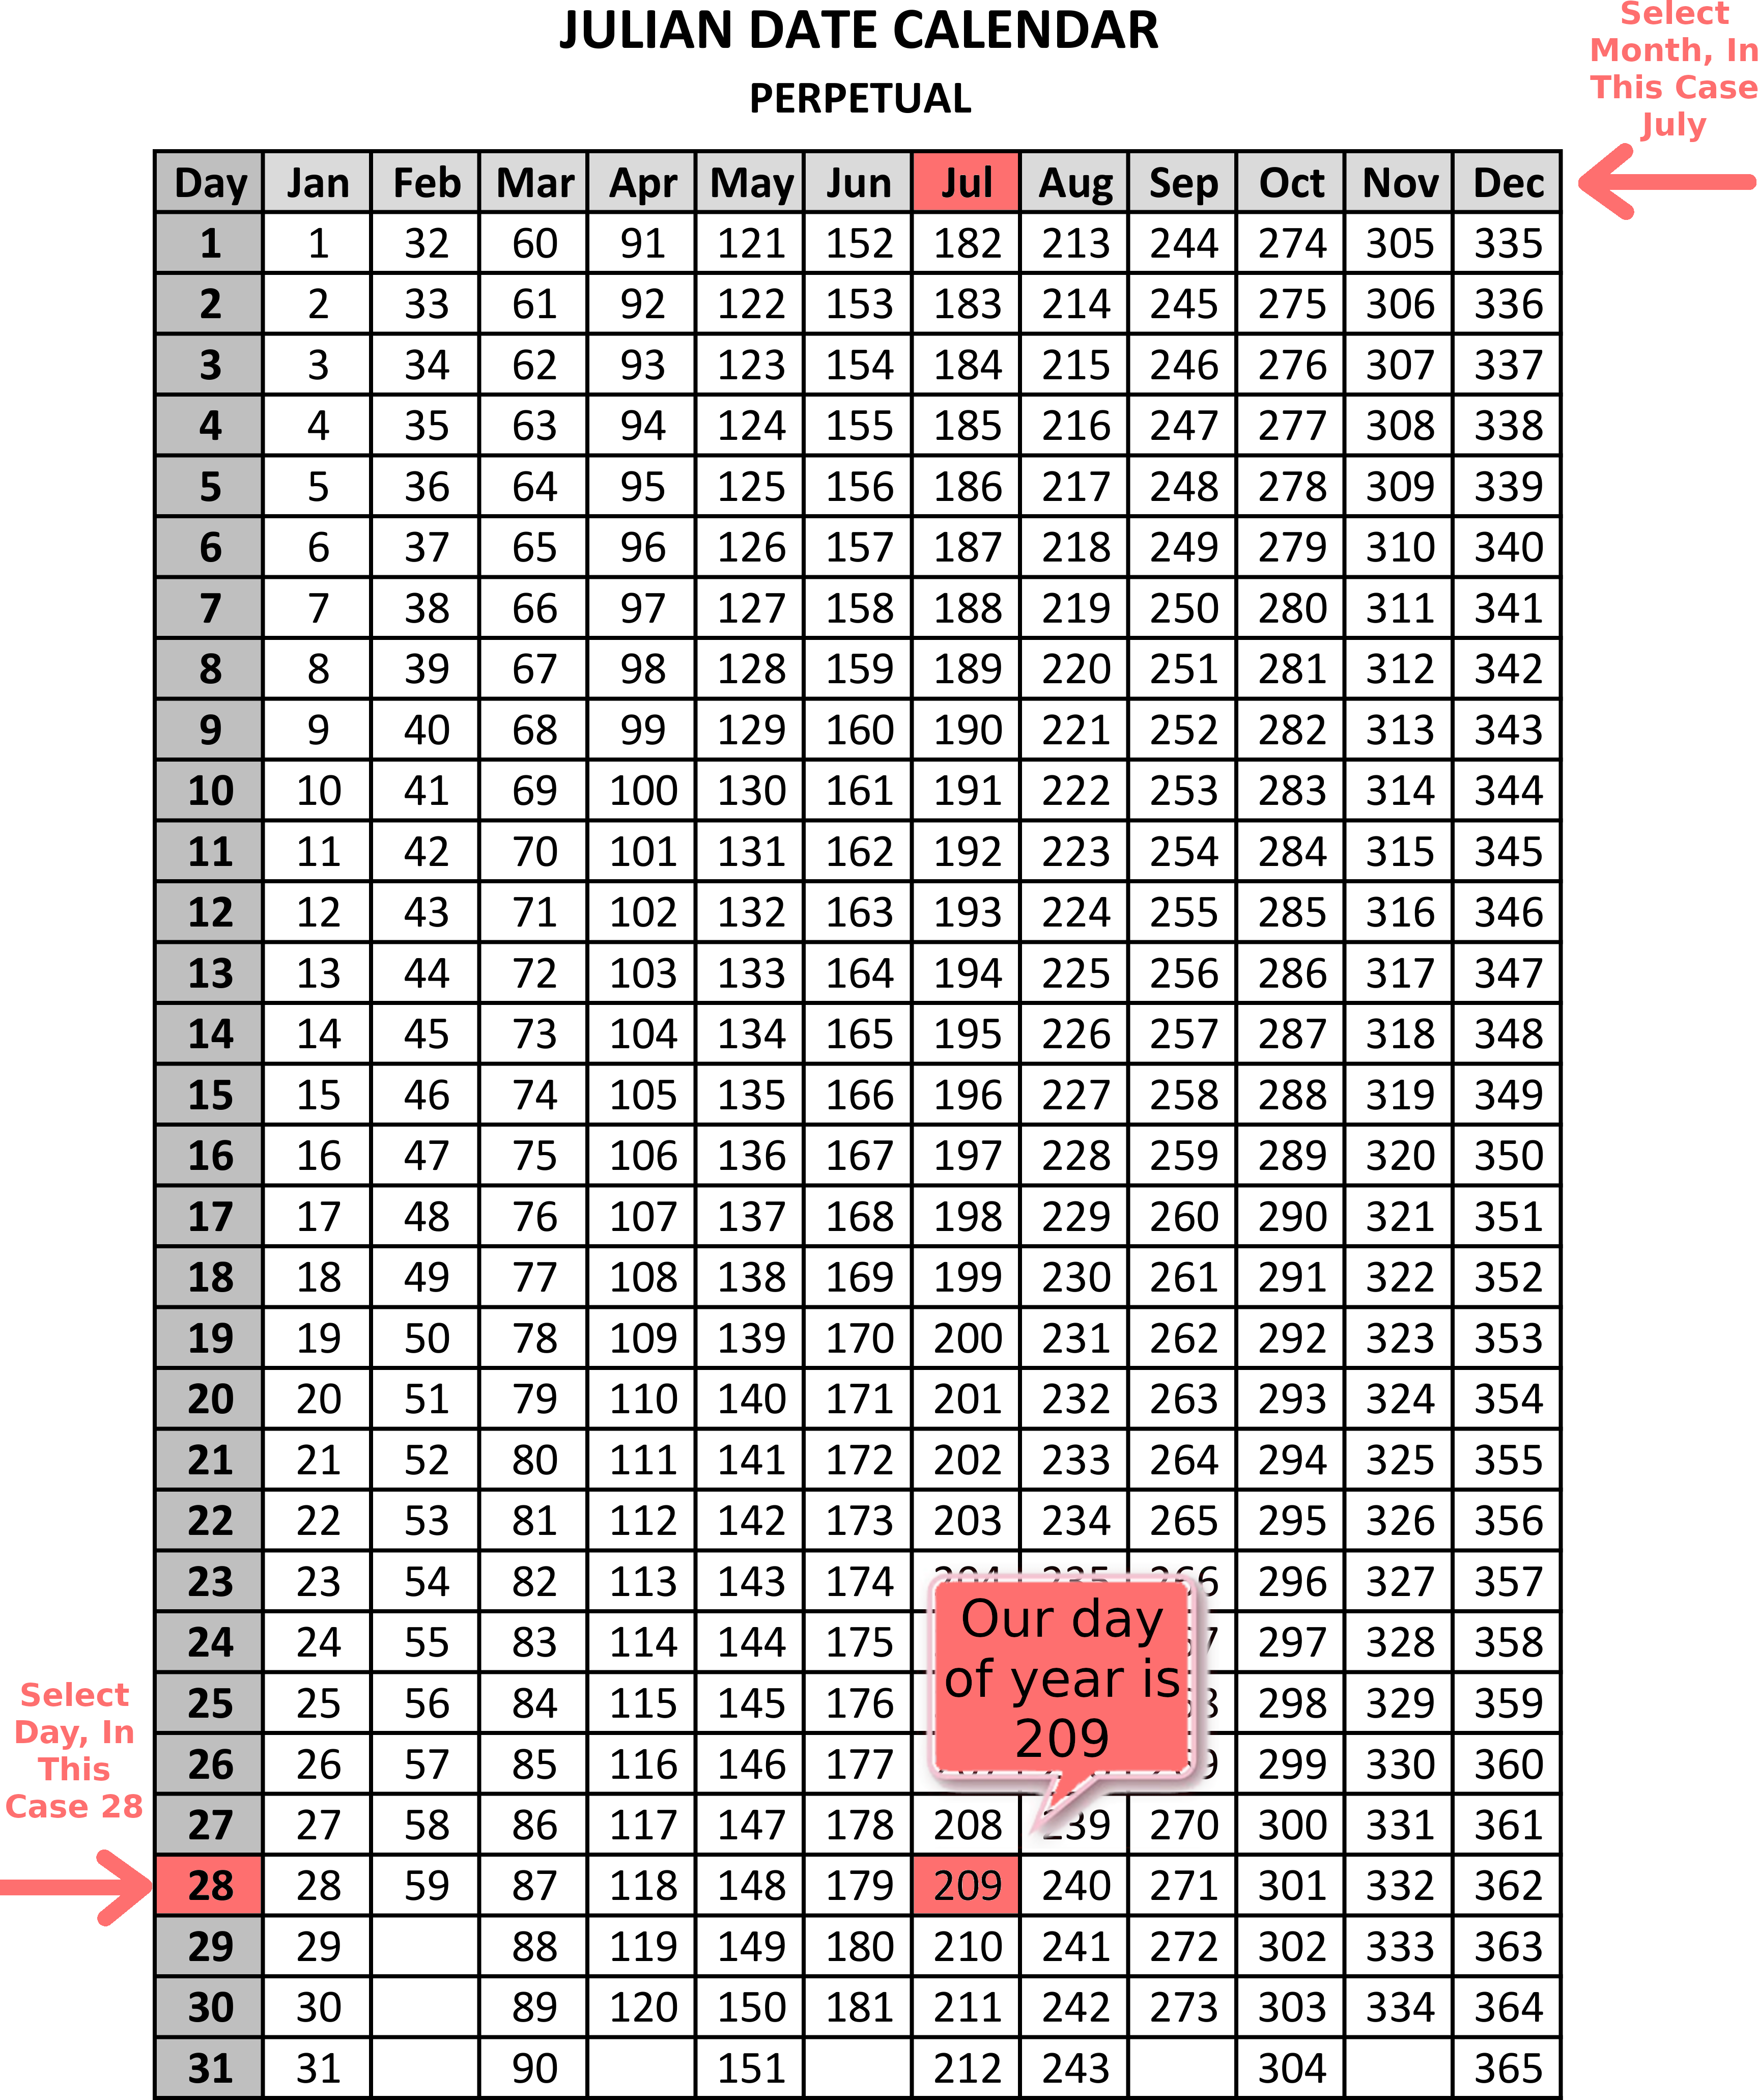
\includegraphics[width=.9\textwidth]{Julian209.png}}

\kulbox{\textbf{NOTE:} You can access the Julian Calendar table anytime by \href{https://jeremydforsythe.github.io/icecream-tutorials/Tutorial4_AccessingRemoteSensingDataWithAppears/Julian_Calendar.png}{clicking this link}. Watch out for leap years!}

14. Access the download page by scrolling to the top of the page, selecting the \textit{Explore} menu and selecting the middle button next to your request, \textit{Download the contents of the request} 
\includegraphics[height=\fontcharht\font`\B]{DownloadButton.png}. Use the Julian calendar and file naming convention listed above to determine what filename we need to download the land surface temperature data for 7/28/2023. There can be multiple files that match the date and layer you requested, in this case there are two. Download both files into the same folder where you saved the DeathValleyNationalPark.zip shapefile.

\centerline{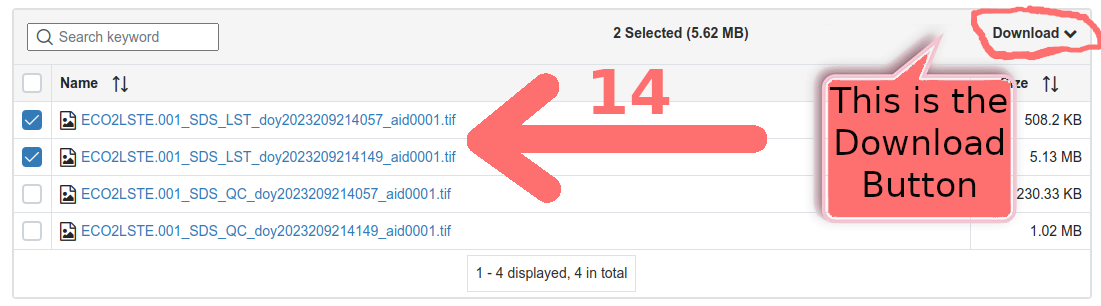
\includegraphics[width=\textwidth]{DownloadInstructions.png}}

15. Cheers! You have now downloaded ECOSTRESS data. In the next tutorial, we will use QGIS to visualize these LST observations.

%%%%%%%%%%%%%%%%%%%%%%%%%%%%%%%%%%%%%%%%%%%%%%%%%%%%%%%%%%%%%%%%%%%%%%%%%%%%%%%%%%% End of Document
\vfill

\begin{tcolorbox}[colback=yellow!5!white,title=\textbf{Datafiles}]
	\addcontentsline{toc}{section}{Datafiles}
	\large
	In case you encountered any issues with the A$\rho\rho$EEARS database, here are copies of the ECOSTRESS GeoTIFF files for Death Valley:
	\begin{enumerate}
		\item \href{https://jeremydforsythe.github.io/icecream-tutorials/Tutorial4_AccessingRemoteSensingDataWithAppears/ECO2LSTE.001_SDS_LST_doy2023209214149_aid0001.tif}{\small ECO2LSTE.001\textunderscore SDS\textunderscore LST\textunderscore doy2023209214149\textunderscore aid0001.tif}
		\item \href{https://jeremydforsythe.github.io/icecream-tutorials/Tutorial4_AccessingRemoteSensingDataWithAppears/ECO2LSTE.001_SDS_LST_doy2023209214057_aid0001.tif}{\small ECO2LSTE.001\textunderscore SDS\textunderscore LST\textunderscore doy2023209214057\textunderscore aid0001.tif}
	\end{enumerate}
\end{tcolorbox}

\hrule

\vspace{1em}

\small \textbf{Recommended Citation:} Forsythe, J.D., G.R. Goldsmith, and J.B. Fisher. 2023. Observing Earth from Above Tutorials. Chapman University. \url{https://jeremydforsythe.github.io/icecream-tutorials/}

\vspace{1em}

This work is supported by funding from NASA ECOSTRESS Mission Grant \#80NSSC23K0309 (I.C.E. C.R.E.A.M.: Integrating Communication of ECOSTRESS Into Community Research, Education, Applications, and Media) and is openly licensed via \href{https://creativecommons.org/licenses/by-nc/4.0/}{CC BY-NC}.

\end{document}
